Tingkat keberhasilan navigasi (\textit{Success Rate}) dan \textit{Collision-Free Rate} (CFR) digunakan sebagai indikator awal untuk mengevaluasi kemampuan sistem dalam mencapai tujuan navigasi tanpa mengalami tabrakan. Kedua metrik ini memberikan gambaran mengenai reliabilitas sistem pada berbagai tingkat kompleksitas lingkungan sebelum dilakukan analisis yang lebih rinci terhadap margin keselamatan, efisiensi navigasi, dan karakteristik pergerakan robot.

\subsection{Success Rate}

Success Rate menunjukkan persentase percobaan yang berhasil mencapai tujuan navigasi dalam batas waktu yang ditentukan tanpa mengalami kegagalan navigasi. Nilai Success Rate pada seluruh skenario ditunjukkan pada Tabel~\ref{tab:success_rate}.

\begin{table}[H]
\centering
\caption{Perbandingan Success Rate pada seluruh skenario pengujian.}
\label{tab:success_rate}
\begin{tabular}{ccc}
\toprule
Skenario & Konfigurasi & Success Rate (\%) \\
\midrule
S1 & Baseline & 100 \\
S2 & Baseline & 100 \\
S3 & Baseline & 65 \\
S4 & Baseline & 0 \\
S5 & Fuzzy & 100 \\
S6 & Fuzzy & 100 \\
S7 & Fuzzy & 100 \\
S8 & Fuzzy & 100 \\
\bottomrule
\end{tabular}
\end{table}

\begin{figure}[H]
\centering
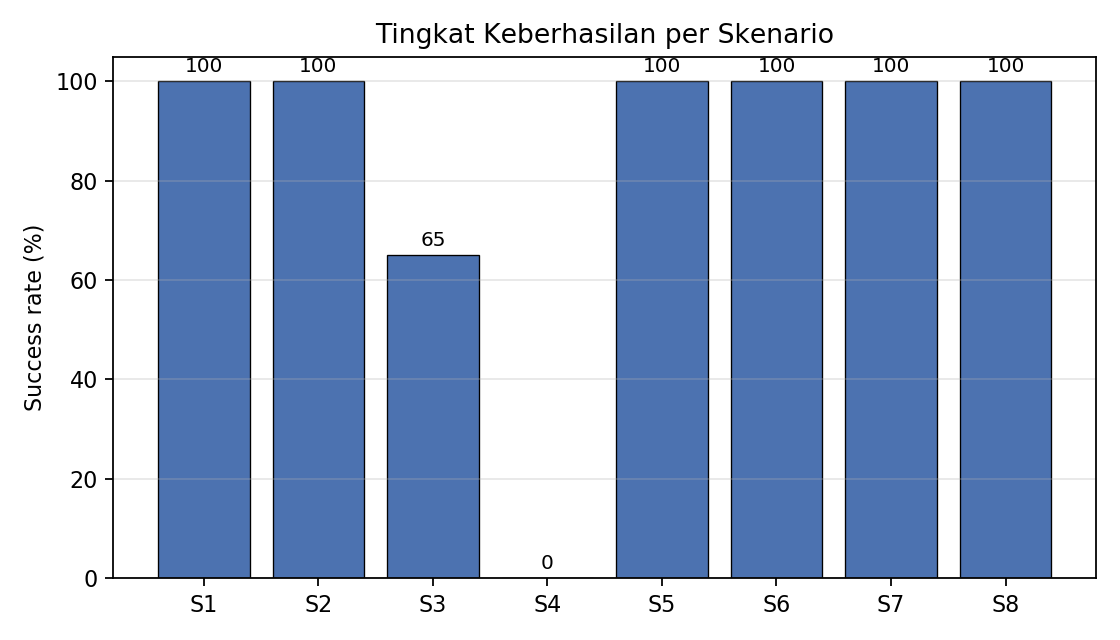
\includegraphics[width=0.6\textwidth]{gambar/4.2_fig_success_rate.png}
\caption{Perbandingan Success Rate pada seluruh skenario pengujian.}
\label{fig:success_rate}
\end{figure}

Hasil pengujian menunjukkan bahwa seluruh percobaan pada S1, S2, S5, dan S6 berhasil mencapai tujuan navigasi. Kondisi ini menunjukkan bahwa baik konfigurasi baseline maupun konfigurasi fuzzy mampu menyelesaikan tugas navigasi secara konsisten pada lingkungan terbuka maupun lingkungan dengan satu obstacle manusia statis.

Perbedaan performa mulai terlihat pada skenario yang memiliki tingkat kompleksitas lebih tinggi. Pada S3, konfigurasi baseline hanya berhasil menyelesaikan 65\% percobaan, sedangkan konfigurasi fuzzy pada S7 mencapai tingkat keberhasilan sebesar 100\%. Peningkatan yang lebih signifikan terlihat pada pasangan S4 dan S8. Seluruh percobaan pada S4 gagal mencapai tujuan sehingga menghasilkan Success Rate sebesar 0\%, sedangkan seluruh percobaan pada S8 berhasil mencapai tujuan dengan Success Rate sebesar 100\%.

Hasil tersebut menunjukkan bahwa metode yang diusulkan memberikan peningkatan reliabilitas navigasi terutama pada lingkungan yang mengandung obstacle berprofil rendah pada area \textit{blind-spot} LiDAR dan obstacle dinamis. Pada kondisi tersebut, informasi tambahan yang diperoleh dari kamera termal memungkinkan sistem mengenali obstacle yang tidak sepenuhnya terdeteksi oleh LiDAR, sementara mekanisme fuzzy membantu robot menyesuaikan perilaku navigasi secara lebih adaptif.

\subsection{Collision-Free Rate}

Selain tingkat keberhasilan navigasi, keamanan sistem juga dievaluasi menggunakan Coll\-ision-Free Rate (CFR). Metrik ini menunjukkan persentase percobaan yang dapat diselesaikan tanpa terjadinya kontak fisik antara robot dan obstacle. Hasil pengujian CFR ditunjukkan pada Tabel\\~\ref{tab:cfr}.

\begin{table}[H]
\centering
\caption{Perbandingan Collision-Free Rate pada seluruh skenario pengujian.}
\label{tab:cfr}
\begin{tabular}{ccc}
\toprule
Skenario & Konfigurasi & CFR (\%) \\
\midrule
S1 & Baseline & 100 \\
S2 & Baseline & 100 \\
S3 & Baseline & 65 \\
S4 & Baseline & 0 \\
S5 & Fuzzy & 100 \\
S6 & Fuzzy & 100 \\
S7 & Fuzzy & 100 \\
S8 & Fuzzy & 100 \\
\bottomrule
\end{tabular}
\end{table}

Nilai CFR menunjukkan pola yang serupa dengan Success Rate. Seluruh percobaan pada S1, S2, S5, dan S6 berhasil diselesaikan tanpa tabrakan. Namun demikian, ketika robot beroperasi pada lingkungan yang lebih kompleks, konfigurasi baseline mengalami penurunan performa yang cukup signifikan.

Pada S3, hanya 65\% percobaan yang dapat diselesaikan tanpa tabrakan. Kondisi yang lebih ekstrem terlihat pada S4, di mana seluruh percobaan mengalami tabrakan sehingga menghasilkan CFR sebesar 0\%. Hasil tersebut menunjukkan bahwa keberadaan obstacle berprofil rendah dan obstacle dinamis menjadi tantangan yang sulit diatasi oleh konfigurasi baseline.

Sebaliknya, konfigurasi fuzzy mempertahankan CFR sebesar 100\% pada seluruh skenario pengujian. Peningkatan ini mengindikasikan bahwa integrasi kamera termal dan mekanisme adaptasi fuzzy mampu meningkatkan kemampuan sistem dalam menghindari obstacle secara konsisten. Dengan memanfaatkan informasi traversability hasil fusi sensor, robot dapat mempertahankan jarak aman yang lebih besar terhadap obstacle sehingga risiko tabrakan dapat diminimalkan.

Temuan pada subbab ini menunjukkan bahwa perbedaan performa antara konfigurasi baseline dan fuzzy relatif kecil pada lingkungan yang sederhana, namun menjadi sangat signifikan ketika robot beroperasi pada lingkungan yang mengandung obstacle berprofil rendah maupun obstacle dinamis. Untuk memahami peningkatan keselamatan navigasi secara lebih rinci, analisis pada subbab berikutnya difokuskan pada evaluasi \textit{minimum clearance} sebagai metrik utama penelitian ini.